% ****************************************************************************************************
\chapter{Causal Loop Diagram -- A qualitative Model}\label{ch:cld}
% ****************************************************************************************************

\begin{flushright}{\slshape    
	We shape our buildings; thereafter, our buildings shape us.} \\ \medskip
	--- Winston Churchill
\end{flushright}

Within this chapter, the crucial interdependencies -- high-leverage interventions and policies -- between the above described classification criteria respectively characteristics are reveled and illustrated using the concepts of system dynamics, more specifically by means of a \ac{CLD} and thereby also answering the \thref{srq2}. System dynamics is an approach to study complexity and was originally developed at the \ac{MIT} by Jay W. \citet{Forrester1961}. John D. \citeauthor{Sterman2000} applied system dynamics to business and organizational problems -- a comprehensive \citep{Sterman2000} as well as brief \citep{Sterman2001} introductory guide is provided. Within this thesis the notation and guidelines provided by John D. \citeauthor{Sterman2000} are used (please refer to the above mentioned sources). The ulterior motive behind \ac{CLD} is the simplification of reality by defining suitable model boundaries. \acp{CLD} \textit{"can never be comprehensive (and you shouldn't try: modeling is the art of simplification). They are also never final, but always provisional"} \citep[p. 166]{Sterman2000}. An important aspect of causal relationships within \acp{CLD} which should always bear in mind, is that the causal relations are modeled ceteris paribus (literally translated as "with other things the same" or "all other things being equal or held constant") \footnote{\textit{"A positive link means that if the cause increases, the effect increases above what it would otherwise have been, and if the cause decreases, the effect decreases below what it would otherwise have been. [\ldots] A negative link means that if the cause increases, the effect decreases below what it would otherwise have been, and if the cause decreases, the effect increases above what it would otherwise have been"} \citep[p. 139]{Sterman2000}.}.

In the beginning of this chapter, the causal relationships for the generic customer segment in the \ac{PaaS} domain are discussed in Section \ref{ch:cld:cs}. Thereafter, interdependencies between the five identified customer segments are presented in Section \ref{ch:cld:csi}. At the end of this chapter, the overall \ac{CLD} is depicted and explained in Section \ref{ch:cld:bp}.

\section{Generic Platform as a Service Customer Segment}\label{ch:cld:cs}

Based on the outcome of the \thref{srq1} and, in addition, the information as well as insights gained through the 23 performed explorative case studies, the below presented relationships in the domain of the generic \ac{PaaS} customer segment were revealed. As mentioned earlier already, this process is by nature iterative and thereby also in alignment with the design cycle introduced by \citet{Hevner2004} respectively \citet{Hevner2007} and the \ac{DSR} methodology process model introduced by \citet{Peffers2007}. Also the evaluation with experts and a focus group was conducted iteratively and the hereafter discussed results represent the final version. Remarkable model changes during the origination process are mentioned.

The heart of the first sub-model -- generic \ac{PaaS} customer segment (cf. Figure \ref{fig:cld_cs}) -- is the actual adoption process. This process is adopted from \citet[p. 18]{Sterman2001} and consists of the two main variables potential <customer segment>\footnote{The wildcard \texttt{<Customer Segment>} respectively \texttt{<customer segment>} represents the five earlier identified customer segments -- IT startup, \ac{SI}, \ac{ISV}, platform customer, and application customer.} and the <customer segment> population which both are influenced by the adoption rate <customer segment> and vice versa. Associated with an increase in the <customer segment> population, the value of favorable word of mouth variable will increase above what it would otherwise have been (and vice versa: if the <customer segment> population decreases, the value of the word of mouth variable will decrease below what it would otherwise have been). In the same vein, an increase respectively decrease in the value of the word of mouth variable increases respectively decrease the value of the adoption rate <customer segment>. To close this cycle, the adoption rate <customer segment> affects the <customer segment> population similarly, an increase in the adoption rate <customer segment> increases the <customer segment> population above what it would otherwise have been, and obvious vice versa. So far, the first self-reinforcing feedback loop (labeled as R\_1\footnote{R\_1: adoption rate <customer segment> -- <customer segment> population -- word of mouth -- adoption rate <customer segment>}) in this model has been described -- \citet[p. 19]{Sterman2001} named this cycle \textit{"contagion loop"}. A self-reinforcing feedback loop will -- without any outside influences -- let all involved variables grow exponentially. Obvious, the <customer segment> population cannot growth exponentially and thus at least one variable out of the self-reinforcing feedback loop needs to be influenced exogenous. In this particular case, the adoption rate <customer segment> is regulated through the variable potential <customer segment>. An increase in the adoption rate <customer segment> will decreases the variable potential <customer segment> below what it would otherwise have been, hence the negative polarity on the link from the adoption rate <customer segment> to the potential <customer segment>. The variable potential <customer segment> itself influences the adoption rate <customer segment> contrary -- a decrease in the number of potential <customer segment> will decrease the number of adopters (adoption rate <customer segment>) below what it would otherwise have been. Due to the fact, that this feedback loop contains one link with a negative polarity, it is a balancing feedback loop (labeled as B\_1\footnote{B\_1: adoption rate <customer segment> -- potential <customer segment> -- adoption rate <customer segment>}), \citet[p. 18]{Sterman2001} named this cycle as follows: \textit{"market saturation"}. This balancing feedback loop prevents the exponential growth of the quantity <customer segment> population and adjusts the adoption rate <customer segment> correspondingly.

\begin{figure}[tb]
	\centering
	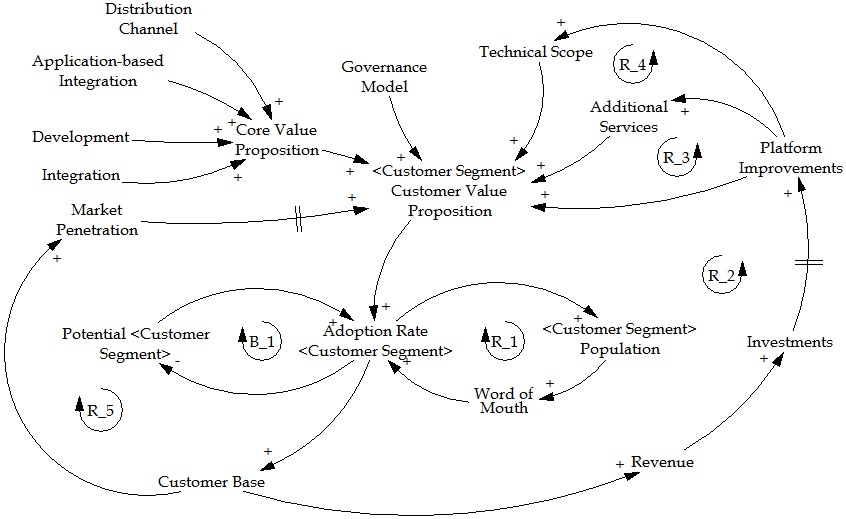
\includegraphics[width=\textwidth]{gfx/cld_customerSegment}
	\caption{Causal Loop Diagram -- Generic PaaS Customer Segment}
	\label{fig:cld_cs}
\end{figure}

In addition to the two above mentioned links to the adoption rate <customer segment>, the main link in the \ac{PaaS} domain is the influence link through the <customer segment> customer value proposition. As discussed earlier, the business model conceptualization proposed by \citet{Johnson2008} emphasizes to provide a dedicated \ac{CVP} for each customer segment to take the different customer needs explicitly into account. Thus, all five identified customer segments receive their own, dedicated \ac{CVP}. The relationship between the <customer segment> customer value proposition and the adoption rate <customer segment> is naturally a link with a positive polarity -- an increase in the <customer segment> customer value proposition will increase the adoption rate <customer segment> above what it would otherwise have been. During the evolution of the qualitative model, the aspect of the \ac{CVP} was discussed quite controversial. It was challenged, if it is necessary to model the \ac{CVP} quintuple, particularly for each customer segment. Finally, the discussion resulted in agreement that the consideration of five different \acp{CVP} is crucial to constitute the causal relationships in the \ac{PaaS} domain.

The <customer segment> customer value proposition itself is influenced sixfold -- through the (1) core value proposition, (2) governance, (3) technical scope, (4) additional services, (5) market penetration, and (6) platform improvements. During the analysis of the 23 explorative case studies (especially in regards to the \ac{CVP}) as well as during the development of the classification scheme, a correlation between the core value proposition and the <customer segment> customer value proposition has been recognized. For the purpose of classifying \ac{PaaS} providers' it was argued that a provider is classified mainly by one characteristic. However, in case of the qualitative model, the core value proposition of a \ac{PaaS} provider is composed of all four identified core value proposition characteristics (cf. Section \ref{ch:sota:cm}). The specific impact of the core value proposition onto the <customer segment> customer value proposition depends on the actual <customer segment> and needs to be further investigated for the transformation into a quantified model.

Moreover, the <customer segment> customer value proposition is influenced by two further classification criteria's -- namely governance and technical scope. Both criteria are mapped onto an ordinal scale, so it is straightforward to model the impact on the <customer segment> customer value proposition. An increase in the value of the technical scope or governance will increase the <customer segment> customer value proposition above what it would otherwise have been. Also here the specific impact of both values onto the <customer segment> customer value proposition depends on the actual <customer segment> and needs to be further investigated for the transformation into a quantified model. The two variables governance and core value proposition (respectively its four influence variables) will remain constant, due to the fact that these variables are not influenced itself by any other variables.

Another point which was discussed during the 	evolution of this qualitative model was how to include the identified revenue streams into the model. Based on the lack of knowledge of user preferences concerning the revenue streams, these are excluded of the model because they cannot be modeled realistic. Further research is necessary to determine which revenue streams are preferred by the \ac{PaaS} stockholders. However, the analysis of the 23 explorative case studies revealed that nearly all \ac{PaaS} providers offer complementary products and especially services, for instance trainings, certifications, and consultancy services. Hence, it is inferred that these complements (henceforth referred to as additional services) influence the <customer segment> customer value proposition favorable. An increase in the value of the additional services variable will increase the value of the <customer segment> customer value proposition above what it would otherwise have been. Once again, the specific impact of the variable additional services onto the <customer segment> customer value proposition depends on the actual <customer segment> and needs to be further investigated for the transformation into a quantified model.

In the opposite direction, the adoption rate <customer segment> influences the variable customer base positive -- an increase in the adoption rate <customer segment> will increase the customer base above what it would otherwise have been. The impacts of the variable customer base are twofold. First, an increase in the variable customer base will increase the variable revenue above what it would otherwise have been. In return, an increase in the variable revenue will increase the value of the variable investments above what it would otherwise have been. Continuing, an increase in the variable investments will increase the variable platform improvements delayed above what it would otherwise have been. The variable platform improvements influences three above already mentioned variables -- <customer segment> customer value proposition, additional services, and technical scope -- and thus three further self-reinforcing feedback loops can be identified (labeled as R\_2\footnote{R\_2: customer base -- revenue -- investments --- platform improvements -- <customer segment> customer value proposition -- adoption rate <customer segment> -- customer base}, R\_3\footnote{R\_3: customer base -- revenue -- investments --- platform improvements -- additional services -- <customer segment> customer value proposition -- adoption rate <customer segment> -- customer base}, and R\_4\footnote{R\_4: customer base -- revenue -- investments --- platform improvements -- technical scope -- <customer segment> customer value proposition -- adoption rate <customer segment> -- customer base}). As already mentioned a couple of time above, the specific impact of the variable platform improvements onto the <customer segment> customer value proposition, additional services, and technical scope depends on the actual <customer segment> and needs to be further investigated for the transformation into a quantified model.

The second impact of the variable customer base concerns the variable market penetration. An increase in the variable customer base will increase the variable market penetration above what it would otherwise have been. Within the 23 explorative case studies, it was remarkable that a company's brand image respectively the company's reputation was an important element of their \ac{CVP}. It is concluded, that this issue will influence the <customer segment> customer value proposition, even though this impact will occur delayed. Hence, an increase in the variable market penetration will increase the variable <customer segment> customer value proposition delayed above what it would otherwise have been. The above described causal relationships constitute the fifth self-reinforcing feedback loop (labeled as R\_5\footnote{R\_5: customer base -- market penetration --- <customer segment> customer value proposition -- adoption rate <customer segment> -- customer base}).

\section{Platform as a Service Customer Segment Interdependencies}\label{ch:cld:csi}

%\begin{figure}[tb]
%	\centering
%	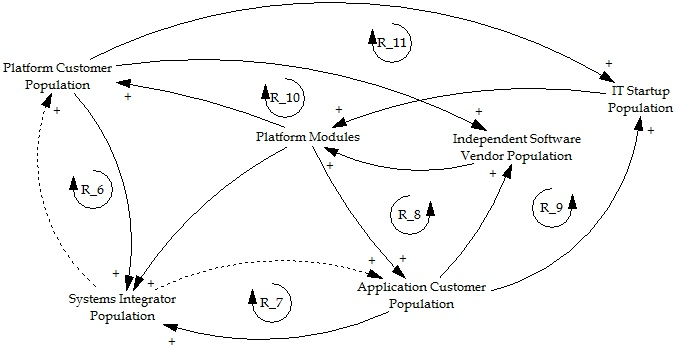
\includegraphics[width=\textwidth]{gfx/cld_customerSegmentInterdependencies}
%	\caption{Causal Loop Diagram -- \ac{PaaS} Customer Segment Interdependencies}
%	\label{fig:cld_csi}
%\end{figure}



\section{The Big Picture}\label{ch:cld:bp}

\begin{itemize}
	\item kein market share der Konkurrenz, da zu umfassend, wird erstmal vernachl�ssig; �ber die initialen potential customers (initial value) kann dies rudiment�r abgebildet werden (new entrants, markts�ttigung, market share competition, marketanteil
	\item keine Kosten, da zu komplex (hosting Standort, Anzahl Developer)
\end{itemize}


